\subsection{Avro [SP]}
\label{subs:avro}

Data should be structured when it is transferred over the network.
Data objects are converted into some form, in which they can be stored or transferred and later be reconstructed in a new environment.
This process is called serialization.
The naive serialization approaches are XML or JSON.
Drawbacks of these formats that they require too much space for storing, because the data is kept it a text form.
The better solution is to use binary format for serialization and Apache Avro is one of the frameworks that use such approach.

Avro differs from the other serialization frameworks in that it does not require the code generation on receivivg.
It even allows to efficiently sort binary-encoded data without deserialization.
Also Avro supports easy schema changes, because it stores both old and new schemas and can associate fields with each other using their names.
This framework provides two types of encoding: binary encoding and using JSON.

Avro uses \textit{schemas} that are defined using JSON.
It needs a schema for serialization and in most cases this schema is transmitted along with the data.
Thus the receiving application does not need to store schemas for deserialization.
However, in some scenarios the transmission of schema is redundant, because both sides have the full schema stored locally.
In this case it is possible to transmitt only a binary representation of serialized objects.

The schema can contain both primitive and complex types.
Primitive types include: \textit{null}, \textit{boolean}, \textit{bytes}, \textit{int}, \textit{long}, \textit{string}, \textit{float} and \textit{double}.
Complex types are: \textit{record}, \textit{array}, \textit{enum}, \textit{union}, \textit{map} and \textit{fixed}.
Listing~\ref{lis:example_avro_schema} illustrates the example schema.
One schema files stores only one schema definition.

\begin{lstlisting}[caption=Avro schema (example), label=lis:example_avro_schema]
{
  "name":"AppInstall",
  "namespace": "example.avro",
  "type":"record",
  "fields":[
     { "name":"id", "type":"long" },
     { "name":"userId", "type":"long" },
     { "name":"time", "type":"long" },
     { "name":"appName", "type":"string" },
     { "name":"packageName", "type":"string" }
  ]
}
\end{lstlisting}

Avro uses an \textit{object container format} for storing objects in a file.
A file has a specified schema, that consists of blocks with synchronization markers between them.
Blocks contain data objects and can be compressed.
Synchronization markers allow to split file for processing it with MapReduce.
Moreover, Avro file comtains metadata section, where it stores a schema.

A file has the following structure: it has a header and one or several file data blocks.
The header contains information about encoding type and file metadata.
Metadata stores the schema and a type of codec that is used for compressing.
'null' codec type means that the data is uncompressed, 'deflate' codec uses the deflate algorithm.
The file data block stores information about the number of objects it contains, their sizes in bytes after compression, the serialized objects themselves and a synchronization marker.
This additional data helps to detect corrupted blocks.

Avro provides a \textit{Remote Procedure Call} (RPC) interface for implementing data exchange between a server and a client.
RPC protocol is defined using JSON.
Its attributes include a \textit{messages} object, that specifies the messages that are exchanged.  
\textit{Message} is a byte sequence, that is transmitted using a transport mechanism.
Transport system sends requests and receives responces.

Transport can have a stateless or stateful design.
\textit{Stateless} means that a server does not store any information about a client state.
The client transmitts all the needed data in every request message.
In \textit{stateful} design the server keeps the persistent client state.
This approaches has two problems.
First, the server should have a mechanism to discard client state at some point.
It is not possible to store the states of all the client for unlimited period of time.
Second, the server should be able to restore the client state in the case of the server crash.
This makes the process of server-side implementation complex comparing to sateless design.
However, stateful design results in better performance.
Figure~\ref{fig:stateful_stateless} represents the stateful and stateless schemas.

\begin{figure}
  \centering
  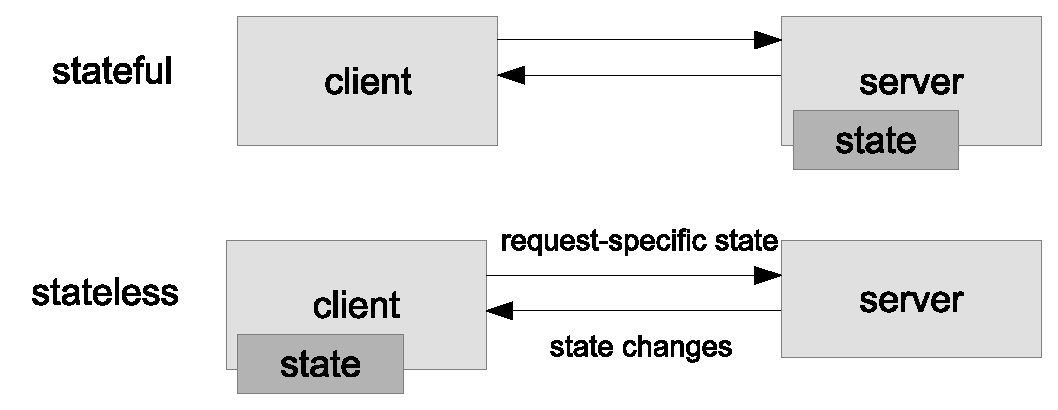
\includegraphics [width=0.7\textwidth]{images/stateful_stateless}
  \caption{Stateless and stateful design}
  \label{fig:stateful_stateless}
\end{figure}

An example of stateless transport method for Avro is HTTP.
In this case all Avro messages share the same URL at an HTTP server.
The 200 (OK) response code should be used by all response messages (normal and error).
Avro sends requests via the POST method.

There is an intermediate layer between messages and transport named \textit{framing}.
The main idea of framing is the partition of each message to a list of buffers.
A buffer contains buffer length followed by buffer data of this length.
Every message consists of one or several buffers.
Framing makes read and write operations more efficient.

Avro uses a handshake procedure before sending any RPC requests and responses.
It is used to make sure that the protocol definition is the same on both the server and the client side.
Only in this case the server and the client can correctly deserialize requests and responces.
To avoid extra network exchanges the server and the client stores recently used protocols in a cache.
Stateless and stateful transport differs in that the former requres a handshake before every request and response.
In contrast, the latter needs only one handshake and for the lifetime of the connection.

The handshake procedure is the following.
The client sends a \textit{HandshakeRequest} in a form \textit{(clientHash=clienthash, clientProtocol=null, serverHash=serverhash)}.
The \textit{clienthash} and the \textit{serverhash} are both the JSON protocol text, hashed with MD5.
The \textit{serverhash} contains data that the client received from the server during the last session.
If it is the first connection to this server the client tries to guess the server's hash.
The server sends in response a \textit{HandshakeResponse}.
If the received \textit{serverhash} is valid and the server knows the corresponding protocol to this client, the response has a form \textit{(match=BOTH, serverProtocol=null, serverHash=null)}.
In this case the connection is confirmed and the server can send a response message.
If the \textit{serverhash} is not valid, but the server knows the client protocol, it answers with \textit{(match=CLIENT, serverProtocol=serverprotocol, serverHash=serverhash)}.
It also allows the server to send the response data to the client.
However, the client must replace its nonvalid \textit{serverhash} data with that received from the server and process the response using the received protocol.
When the server is not aware of the client's protocol it received, it response with \textit{(match=NONE)}. 
Then the client re-sends its request extended by \textit{clientProtocol} value and the server response with \textit{(match=BOTH)}.

To determine the identity of the schemas stored on the client and the server side, Avro uses \textit{Parsing Canonical Form}.
It is a transformation, that removes data, irrelevant for the comparison, and normalizes the JSON text.
This canonical form can be used to create a fingerprint (an integer that serves as a unique id for a schema). 

 

